% Created by tikzDevice version 0.6.2 on 2012-04-21 14:58:22
% !TEX encoding = UTF-8 Unicode
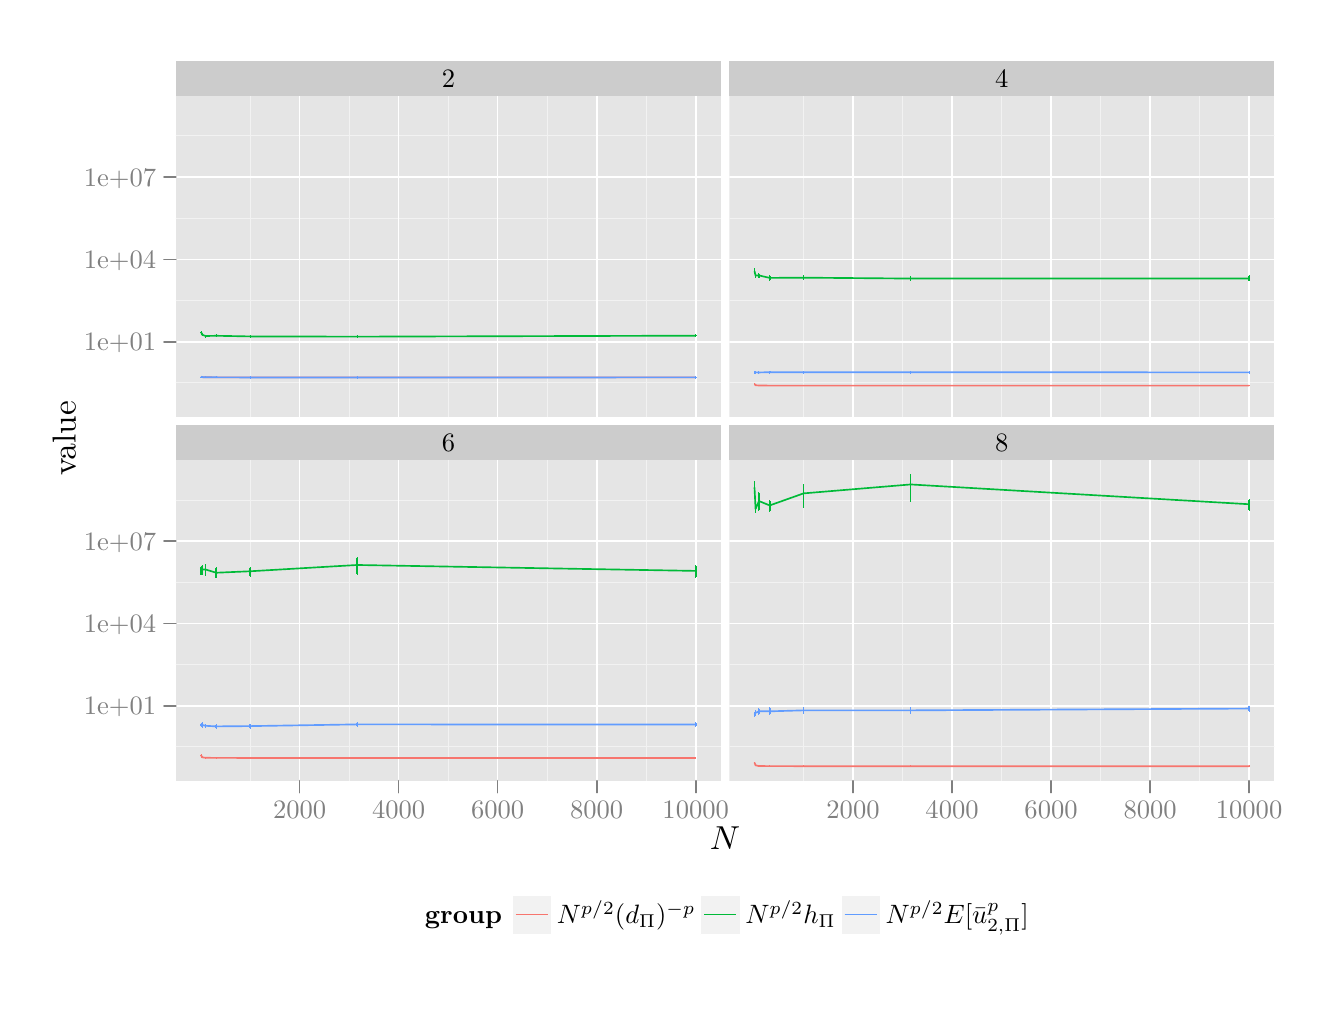
\begin{tikzpicture}[x=1pt,y=1pt]
\definecolor[named]{drawColor}{rgb}{0.00,0.00,0.00}
\definecolor[named]{fillColor}{rgb}{1.00,1.00,1.00}
\fill[color=fillColor,fill opacity=0.00,] (0,0) rectangle (462.53,346.90);
\begin{scope}
\path[clip] (  0.00,  0.00) rectangle (462.53,346.90);
\definecolor[named]{drawColor}{rgb}{0.41,0.16,0.58}
\end{scope}
\begin{scope}
\path[clip] (  0.00,  0.00) rectangle (462.53,346.90);
\definecolor[named]{drawColor}{rgb}{0.41,0.16,0.58}
\end{scope}
\begin{scope}
\path[clip] (  0.00,  0.00) rectangle (462.53,346.90);
\definecolor[named]{drawColor}{rgb}{0.41,0.16,0.58}
\end{scope}
\begin{scope}
\path[clip] (  0.00,  0.00) rectangle (462.53,346.90);
\definecolor[named]{drawColor}{rgb}{0.41,0.16,0.58}
\end{scope}
\begin{scope}
\path[clip] (  0.00,  0.00) rectangle (462.53,346.90);
\definecolor[named]{drawColor}{rgb}{0.41,0.16,0.58}
\end{scope}
\begin{scope}
\path[clip] (  0.00,  0.00) rectangle (462.53,346.90);
\definecolor[named]{drawColor}{rgb}{0.41,0.16,0.58}
\end{scope}
\begin{scope}
\path[clip] (  0.00,  0.00) rectangle (462.53,346.90);
\definecolor[named]{drawColor}{rgb}{0.41,0.16,0.58}
\end{scope}
\begin{scope}
\path[clip] (  0.00,  0.00) rectangle (462.53,346.90);
\definecolor[named]{drawColor}{rgb}{0.41,0.16,0.58}
\end{scope}
\begin{scope}
\path[clip] ( 53.55,206.31) rectangle (250.51,322.22);
\definecolor[named]{drawColor}{rgb}{0.41,0.16,0.58}
\end{scope}
\begin{scope}
\path[clip] (  0.00,  0.00) rectangle (462.53,346.90);
\definecolor[named]{drawColor}{rgb}{0.41,0.16,0.58}
\end{scope}
\begin{scope}
\path[clip] (253.52,206.31) rectangle (450.48,322.22);
\definecolor[named]{drawColor}{rgb}{0.41,0.16,0.58}
\end{scope}
\begin{scope}
\path[clip] (  0.00,  0.00) rectangle (462.53,346.90);
\definecolor[named]{drawColor}{rgb}{0.41,0.16,0.58}
\end{scope}
\begin{scope}
\path[clip] ( 53.55, 74.76) rectangle (250.51,190.67);
\definecolor[named]{drawColor}{rgb}{0.41,0.16,0.58}
\end{scope}
\begin{scope}
\path[clip] (  0.00,  0.00) rectangle (462.53,346.90);
\definecolor[named]{drawColor}{rgb}{0.41,0.16,0.58}
\end{scope}
\begin{scope}
\path[clip] (253.52, 74.76) rectangle (450.48,190.67);
\definecolor[named]{drawColor}{rgb}{0.41,0.16,0.58}
\end{scope}
\begin{scope}
\path[clip] (  0.00,  0.00) rectangle (462.53,346.90);
\definecolor[named]{drawColor}{rgb}{0.41,0.16,0.58}
\end{scope}
\begin{scope}
\path[clip] (  0.00,  0.00) rectangle (462.53,346.90);
\definecolor[named]{drawColor}{rgb}{0.41,0.16,0.58}
\end{scope}
\begin{scope}
\path[clip] (  0.00,  0.00) rectangle (462.53,346.90);
\definecolor[named]{drawColor}{rgb}{0.41,0.16,0.58}
\end{scope}
\begin{scope}
\path[clip] (  0.00,  0.00) rectangle (462.53,346.90);
\definecolor[named]{drawColor}{rgb}{0.41,0.16,0.58}
\end{scope}
\begin{scope}
\path[clip] (  0.00,  0.00) rectangle (462.53,346.90);
\definecolor[named]{drawColor}{rgb}{0.41,0.16,0.58}
\end{scope}
\begin{scope}
\path[clip] (  0.00,  0.00) rectangle (462.53,346.90);
\definecolor[named]{drawColor}{rgb}{0.41,0.16,0.58}
\end{scope}
\begin{scope}
\path[clip] (  0.00,  0.00) rectangle (462.53,346.90);
\definecolor[named]{drawColor}{rgb}{0.41,0.16,0.58}
\end{scope}
\begin{scope}
\path[clip] (  0.00,  0.00) rectangle (462.53,346.90);
\definecolor[named]{drawColor}{rgb}{0.41,0.16,0.58}
\end{scope}
\begin{scope}
\path[clip] (  0.00,  0.00) rectangle (462.53,346.90);
\definecolor[named]{drawColor}{rgb}{0.41,0.16,0.58}
\end{scope}
\begin{scope}
\path[clip] (  0.00,  0.00) rectangle (462.53,346.90);
\definecolor[named]{drawColor}{rgb}{0.41,0.16,0.58}
\end{scope}
\begin{scope}
\path[clip] (  0.00,  0.00) rectangle (462.53,346.90);
\definecolor[named]{drawColor}{rgb}{0.41,0.16,0.58}
\end{scope}
\begin{scope}
\path[clip] (  0.00,  0.00) rectangle (462.53,346.90);
\definecolor[named]{drawColor}{rgb}{0.41,0.16,0.58}
\end{scope}
\begin{scope}
\path[clip] (  0.00,  0.00) rectangle (462.53,346.90);
\definecolor[named]{drawColor}{rgb}{0.41,0.16,0.58}
\end{scope}
\begin{scope}
\path[clip] (  0.00,  0.00) rectangle (462.53,346.90);
\definecolor[named]{drawColor}{rgb}{0.41,0.16,0.58}
\end{scope}
\begin{scope}
\path[clip] (  0.00,  0.00) rectangle (462.53,346.90);
\definecolor[named]{drawColor}{rgb}{0.41,0.16,0.58}
\end{scope}
\begin{scope}
\path[clip] (  0.00,  0.00) rectangle (462.53,346.90);
\definecolor[named]{drawColor}{rgb}{0.41,0.16,0.58}
\end{scope}
\begin{scope}
\path[clip] (  0.00,  0.00) rectangle (462.53,346.90);
\definecolor[named]{drawColor}{rgb}{0.41,0.16,0.58}
\end{scope}
\begin{scope}
\path[clip] (  0.00,  0.00) rectangle (462.53,346.90);
\definecolor[named]{drawColor}{rgb}{0.41,0.16,0.58}
\end{scope}
\begin{scope}
\path[clip] (  0.00,  0.00) rectangle (462.53,346.90);
\definecolor[named]{drawColor}{rgb}{0.41,0.16,0.58}
\end{scope}
\begin{scope}
\path[clip] (  0.00,  0.00) rectangle (462.53,346.90);
\definecolor[named]{drawColor}{rgb}{0.41,0.16,0.58}
\end{scope}
\begin{scope}
\path[clip] (  0.00,  0.00) rectangle (462.53,346.90);
\definecolor[named]{drawColor}{rgb}{0.41,0.16,0.58}
\end{scope}
\begin{scope}
\path[clip] (  0.00,  0.00) rectangle (462.53,346.90);
\definecolor[named]{drawColor}{rgb}{0.41,0.16,0.58}
\end{scope}
\begin{scope}
\path[clip] (  0.00,  0.00) rectangle (462.53,346.90);
\definecolor[named]{drawColor}{rgb}{0.41,0.16,0.58}
\end{scope}
\begin{scope}
\path[clip] (  0.00,  0.00) rectangle (462.53,346.90);
\definecolor[named]{drawColor}{rgb}{0.41,0.16,0.58}
\end{scope}
\begin{scope}
\path[clip] (  0.00,  0.00) rectangle (462.53,346.90);
\definecolor[named]{drawColor}{rgb}{0.41,0.16,0.58}
\end{scope}
\begin{scope}
\path[clip] (  0.00,  0.00) rectangle (462.53,346.90);
\definecolor[named]{drawColor}{rgb}{0.41,0.16,0.58}
\end{scope}
\begin{scope}
\path[clip] (  0.00,  0.00) rectangle (462.53,346.90);
\definecolor[named]{drawColor}{rgb}{0.41,0.16,0.58}
\end{scope}
\begin{scope}
\path[clip] (  0.00,  0.00) rectangle (462.53,346.90);
\definecolor[named]{drawColor}{rgb}{0.41,0.16,0.58}
\end{scope}
\begin{scope}
\path[clip] (  0.00,  0.00) rectangle (462.53,346.90);
\definecolor[named]{drawColor}{rgb}{0.41,0.16,0.58}
\end{scope}
\begin{scope}
\path[clip] (  0.00,  0.00) rectangle (462.53,346.90);
\definecolor[named]{drawColor}{rgb}{0.41,0.16,0.58}
\end{scope}
\begin{scope}
\path[clip] (  0.00,  0.00) rectangle (462.53,346.90);
\definecolor[named]{drawColor}{rgb}{0.41,0.16,0.58}
\end{scope}
\begin{scope}
\path[clip] (  0.00,  0.00) rectangle (462.53,346.90);
\definecolor[named]{drawColor}{rgb}{0.41,0.16,0.58}
\end{scope}
\begin{scope}
\path[clip] (  0.00,  0.00) rectangle (462.53,346.90);
\definecolor[named]{drawColor}{rgb}{0.41,0.16,0.58}
\end{scope}
\begin{scope}
\path[clip] (  0.00,  0.00) rectangle (462.53,346.90);
\definecolor[named]{drawColor}{rgb}{0.41,0.16,0.58}
\definecolor[named]{fillColor}{rgb}{1.00,1.00,1.00}

\draw[fill=fillColor,draw opacity=0.00,] (  0.00,  0.00) rectangle (462.53,346.90);
\end{scope}
\begin{scope}
\path[clip] (  0.00,  0.00) rectangle (462.53,346.90);
\definecolor[named]{drawColor}{rgb}{0.41,0.16,0.58}
\end{scope}
\begin{scope}
\path[clip] ( 53.55,206.31) rectangle (250.51,322.22);
\definecolor[named]{drawColor}{rgb}{0.41,0.16,0.58}
\definecolor[named]{fillColor}{rgb}{0.90,0.90,0.90}

\draw[fill=fillColor,draw opacity=0.00,] ( 53.55,206.31) rectangle (250.51,322.22);
\definecolor[named]{drawColor}{rgb}{0.95,0.95,0.95}

\draw[color=drawColor,line width= 0.3pt,line cap=round,line join=round,fill opacity=0.00,] ( 53.55,218.56) --
	(250.51,218.56);

\draw[color=drawColor,line width= 0.3pt,line cap=round,line join=round,fill opacity=0.00,] ( 53.55,248.31) --
	(250.51,248.31);

\draw[color=drawColor,line width= 0.3pt,line cap=round,line join=round,fill opacity=0.00,] ( 53.55,278.05) --
	(250.51,278.05);

\draw[color=drawColor,line width= 0.3pt,line cap=round,line join=round,fill opacity=0.00,] ( 53.55,307.80) --
	(250.51,307.80);

\draw[color=drawColor,line width= 0.3pt,line cap=round,line join=round,fill opacity=0.00,] ( 80.38,206.31) --
	( 80.38,322.22);

\draw[color=drawColor,line width= 0.3pt,line cap=round,line join=round,fill opacity=0.00,] (116.16,206.31) --
	(116.16,322.22);

\draw[color=drawColor,line width= 0.3pt,line cap=round,line join=round,fill opacity=0.00,] (151.94,206.31) --
	(151.94,322.22);

\draw[color=drawColor,line width= 0.3pt,line cap=round,line join=round,fill opacity=0.00,] (187.72,206.31) --
	(187.72,322.22);

\draw[color=drawColor,line width= 0.3pt,line cap=round,line join=round,fill opacity=0.00,] (223.50,206.31) --
	(223.50,322.22);
\definecolor[named]{drawColor}{rgb}{1.00,1.00,1.00}

\draw[color=drawColor,line width= 0.6pt,line cap=round,line join=round,fill opacity=0.00,] ( 53.55,233.43) --
	(250.51,233.43);

\draw[color=drawColor,line width= 0.6pt,line cap=round,line join=round,fill opacity=0.00,] ( 53.55,263.18) --
	(250.51,263.18);

\draw[color=drawColor,line width= 0.6pt,line cap=round,line join=round,fill opacity=0.00,] ( 53.55,292.92) --
	(250.51,292.92);

\draw[color=drawColor,line width= 0.6pt,line cap=round,line join=round,fill opacity=0.00,] ( 98.27,206.31) --
	( 98.27,322.22);

\draw[color=drawColor,line width= 0.6pt,line cap=round,line join=round,fill opacity=0.00,] (134.05,206.31) --
	(134.05,322.22);

\draw[color=drawColor,line width= 0.6pt,line cap=round,line join=round,fill opacity=0.00,] (169.83,206.31) --
	(169.83,322.22);

\draw[color=drawColor,line width= 0.6pt,line cap=round,line join=round,fill opacity=0.00,] (205.61,206.31) --
	(205.61,322.22);

\draw[color=drawColor,line width= 0.6pt,line cap=round,line join=round,fill opacity=0.00,] (241.39,206.31) --
	(241.39,322.22);
\definecolor[named]{drawColor}{rgb}{0.97,0.46,0.43}

\draw[color=drawColor,line width= 0.6pt,line join=round,fill opacity=0.00,] ( 62.67,220.79) --
	( 63.05,220.61) --
	( 64.28,220.56) --
	( 68.15,220.54) --
	( 80.38,220.54) --
	(119.06,220.53) --
	(241.39,220.53);
\definecolor[named]{drawColor}{rgb}{0.00,0.73,0.22}

\draw[color=drawColor,line width= 0.6pt,line join=round,fill opacity=0.00,] ( 62.67,236.88) --
	( 63.05,235.96) --
	( 64.28,235.48) --
	( 68.15,235.56) --
	( 80.38,235.33) --
	(119.06,235.25) --
	(241.39,235.60);
\definecolor[named]{drawColor}{rgb}{0.38,0.61,1.00}

\draw[color=drawColor,line width= 0.6pt,line join=round,fill opacity=0.00,] ( 62.67,220.72) --
	( 63.05,220.61) --
	( 64.28,220.59) --
	( 68.15,220.55) --
	( 80.38,220.50) --
	(119.06,220.47) --
	(241.39,220.53);
\definecolor[named]{drawColor}{rgb}{0.97,0.46,0.43}

\draw[color=drawColor,line width= 0.6pt,line join=round,fill opacity=0.00,] ( 62.50,220.80) --
	( 62.84,220.80);

\draw[color=drawColor,line width= 0.6pt,line join=round,fill opacity=0.00,] ( 62.67,220.80) --
	( 62.67,220.79);

\draw[color=drawColor,line width= 0.6pt,line join=round,fill opacity=0.00,] ( 62.50,220.79) --
	( 62.84,220.79);

\draw[color=drawColor,line width= 0.6pt,line join=round,fill opacity=0.00,] ( 62.88,220.61) --
	( 63.22,220.61);

\draw[color=drawColor,line width= 0.6pt,line join=round,fill opacity=0.00,] ( 63.05,220.61) --
	( 63.05,220.60);

\draw[color=drawColor,line width= 0.6pt,line join=round,fill opacity=0.00,] ( 62.88,220.60) --
	( 63.22,220.60);

\draw[color=drawColor,line width= 0.6pt,line join=round,fill opacity=0.00,] ( 64.11,220.56) --
	( 64.45,220.56);

\draw[color=drawColor,line width= 0.6pt,line join=round,fill opacity=0.00,] ( 64.28,220.56) --
	( 64.28,220.55);

\draw[color=drawColor,line width= 0.6pt,line join=round,fill opacity=0.00,] ( 64.11,220.55) --
	( 64.45,220.55);

\draw[color=drawColor,line width= 0.6pt,line join=round,fill opacity=0.00,] ( 67.98,220.54) --
	( 68.32,220.54);

\draw[color=drawColor,line width= 0.6pt,line join=round,fill opacity=0.00,] ( 68.15,220.54) --
	( 68.15,220.54);

\draw[color=drawColor,line width= 0.6pt,line join=round,fill opacity=0.00,] ( 67.98,220.54) --
	( 68.32,220.54);

\draw[color=drawColor,line width= 0.6pt,line join=round,fill opacity=0.00,] ( 80.21,220.54) --
	( 80.55,220.54);

\draw[color=drawColor,line width= 0.6pt,line join=round,fill opacity=0.00,] ( 80.38,220.54) --
	( 80.38,220.53);

\draw[color=drawColor,line width= 0.6pt,line join=round,fill opacity=0.00,] ( 80.21,220.53) --
	( 80.55,220.53);

\draw[color=drawColor,line width= 0.6pt,line join=round,fill opacity=0.00,] (118.89,220.53) --
	(119.23,220.53);

\draw[color=drawColor,line width= 0.6pt,line join=round,fill opacity=0.00,] (119.06,220.53) --
	(119.06,220.53);

\draw[color=drawColor,line width= 0.6pt,line join=round,fill opacity=0.00,] (118.89,220.53) --
	(119.23,220.53);

\draw[color=drawColor,line width= 0.6pt,line join=round,fill opacity=0.00,] (241.22,220.53) --
	(241.56,220.53);

\draw[color=drawColor,line width= 0.6pt,line join=round,fill opacity=0.00,] (241.39,220.53) --
	(241.39,220.53);

\draw[color=drawColor,line width= 0.6pt,line join=round,fill opacity=0.00,] (241.22,220.53) --
	(241.56,220.53);
\definecolor[named]{drawColor}{rgb}{0.00,0.73,0.22}

\draw[color=drawColor,line width= 0.6pt,line join=round,fill opacity=0.00,] ( 62.50,237.10) --
	( 62.84,237.10);

\draw[color=drawColor,line width= 0.6pt,line join=round,fill opacity=0.00,] ( 62.67,237.10) --
	( 62.67,236.66);

\draw[color=drawColor,line width= 0.6pt,line join=round,fill opacity=0.00,] ( 62.50,236.66) --
	( 62.84,236.66);

\draw[color=drawColor,line width= 0.6pt,line join=round,fill opacity=0.00,] ( 62.88,236.19) --
	( 63.22,236.19);

\draw[color=drawColor,line width= 0.6pt,line join=round,fill opacity=0.00,] ( 63.05,236.19) --
	( 63.05,235.73);

\draw[color=drawColor,line width= 0.6pt,line join=round,fill opacity=0.00,] ( 62.88,235.73) --
	( 63.22,235.73);

\draw[color=drawColor,line width= 0.6pt,line join=round,fill opacity=0.00,] ( 64.11,235.71) --
	( 64.45,235.71);

\draw[color=drawColor,line width= 0.6pt,line join=round,fill opacity=0.00,] ( 64.28,235.71) --
	( 64.28,235.24);

\draw[color=drawColor,line width= 0.6pt,line join=round,fill opacity=0.00,] ( 64.11,235.24) --
	( 64.45,235.24);

\draw[color=drawColor,line width= 0.6pt,line join=round,fill opacity=0.00,] ( 67.98,235.79) --
	( 68.32,235.79);

\draw[color=drawColor,line width= 0.6pt,line join=round,fill opacity=0.00,] ( 68.15,235.79) --
	( 68.15,235.36);

\draw[color=drawColor,line width= 0.6pt,line join=round,fill opacity=0.00,] ( 67.98,235.36) --
	( 68.32,235.36);

\draw[color=drawColor,line width= 0.6pt,line join=round,fill opacity=0.00,] ( 80.21,235.57) --
	( 80.55,235.57);

\draw[color=drawColor,line width= 0.6pt,line join=round,fill opacity=0.00,] ( 80.38,235.57) --
	( 80.38,235.11);

\draw[color=drawColor,line width= 0.6pt,line join=round,fill opacity=0.00,] ( 80.21,235.11) --
	( 80.55,235.11);

\draw[color=drawColor,line width= 0.6pt,line join=round,fill opacity=0.00,] (118.89,235.47) --
	(119.23,235.47);

\draw[color=drawColor,line width= 0.6pt,line join=round,fill opacity=0.00,] (119.06,235.47) --
	(119.06,235.04);

\draw[color=drawColor,line width= 0.6pt,line join=round,fill opacity=0.00,] (118.89,235.04) --
	(119.23,235.04);

\draw[color=drawColor,line width= 0.6pt,line join=round,fill opacity=0.00,] (241.22,235.84) --
	(241.56,235.84);

\draw[color=drawColor,line width= 0.6pt,line join=round,fill opacity=0.00,] (241.39,235.84) --
	(241.39,235.37);

\draw[color=drawColor,line width= 0.6pt,line join=round,fill opacity=0.00,] (241.22,235.37) --
	(241.56,235.37);
\definecolor[named]{drawColor}{rgb}{0.38,0.61,1.00}

\draw[color=drawColor,line width= 0.6pt,line join=round,fill opacity=0.00,] ( 62.50,220.84) --
	( 62.84,220.84);

\draw[color=drawColor,line width= 0.6pt,line join=round,fill opacity=0.00,] ( 62.67,220.84) --
	( 62.67,220.60);

\draw[color=drawColor,line width= 0.6pt,line join=round,fill opacity=0.00,] ( 62.50,220.60) --
	( 62.84,220.60);

\draw[color=drawColor,line width= 0.6pt,line join=round,fill opacity=0.00,] ( 62.88,220.74) --
	( 63.22,220.74);

\draw[color=drawColor,line width= 0.6pt,line join=round,fill opacity=0.00,] ( 63.05,220.74) --
	( 63.05,220.50);

\draw[color=drawColor,line width= 0.6pt,line join=round,fill opacity=0.00,] ( 62.88,220.50) --
	( 63.22,220.50);

\draw[color=drawColor,line width= 0.6pt,line join=round,fill opacity=0.00,] ( 64.11,220.71) --
	( 64.45,220.71);

\draw[color=drawColor,line width= 0.6pt,line join=round,fill opacity=0.00,] ( 64.28,220.71) --
	( 64.28,220.46);

\draw[color=drawColor,line width= 0.6pt,line join=round,fill opacity=0.00,] ( 64.11,220.46) --
	( 64.45,220.46);

\draw[color=drawColor,line width= 0.6pt,line join=round,fill opacity=0.00,] ( 67.98,220.67) --
	( 68.32,220.67);

\draw[color=drawColor,line width= 0.6pt,line join=round,fill opacity=0.00,] ( 68.15,220.67) --
	( 68.15,220.43);

\draw[color=drawColor,line width= 0.6pt,line join=round,fill opacity=0.00,] ( 67.98,220.43) --
	( 68.32,220.43);

\draw[color=drawColor,line width= 0.6pt,line join=round,fill opacity=0.00,] ( 80.21,220.62) --
	( 80.55,220.62);

\draw[color=drawColor,line width= 0.6pt,line join=round,fill opacity=0.00,] ( 80.38,220.62) --
	( 80.38,220.38);

\draw[color=drawColor,line width= 0.6pt,line join=round,fill opacity=0.00,] ( 80.21,220.38) --
	( 80.55,220.38);

\draw[color=drawColor,line width= 0.6pt,line join=round,fill opacity=0.00,] (118.89,220.58) --
	(119.23,220.58);

\draw[color=drawColor,line width= 0.6pt,line join=round,fill opacity=0.00,] (119.06,220.58) --
	(119.06,220.35);

\draw[color=drawColor,line width= 0.6pt,line join=round,fill opacity=0.00,] (118.89,220.35) --
	(119.23,220.35);

\draw[color=drawColor,line width= 0.6pt,line join=round,fill opacity=0.00,] (241.22,220.64) --
	(241.56,220.64);

\draw[color=drawColor,line width= 0.6pt,line join=round,fill opacity=0.00,] (241.39,220.64) --
	(241.39,220.41);

\draw[color=drawColor,line width= 0.6pt,line join=round,fill opacity=0.00,] (241.22,220.41) --
	(241.56,220.41);
\end{scope}
\begin{scope}
\path[clip] (  0.00,  0.00) rectangle (462.53,346.90);
\definecolor[named]{drawColor}{rgb}{0.41,0.16,0.58}
\end{scope}
\begin{scope}
\path[clip] (253.52,206.31) rectangle (450.48,322.22);
\definecolor[named]{drawColor}{rgb}{0.41,0.16,0.58}
\definecolor[named]{fillColor}{rgb}{0.90,0.90,0.90}

\draw[fill=fillColor,draw opacity=0.00,] (253.52,206.31) rectangle (450.48,322.22);
\definecolor[named]{drawColor}{rgb}{0.95,0.95,0.95}

\draw[color=drawColor,line width= 0.3pt,line cap=round,line join=round,fill opacity=0.00,] (253.52,218.56) --
	(450.48,218.56);

\draw[color=drawColor,line width= 0.3pt,line cap=round,line join=round,fill opacity=0.00,] (253.52,248.31) --
	(450.48,248.31);

\draw[color=drawColor,line width= 0.3pt,line cap=round,line join=round,fill opacity=0.00,] (253.52,278.05) --
	(450.48,278.05);

\draw[color=drawColor,line width= 0.3pt,line cap=round,line join=round,fill opacity=0.00,] (253.52,307.80) --
	(450.48,307.80);

\draw[color=drawColor,line width= 0.3pt,line cap=round,line join=round,fill opacity=0.00,] (280.35,206.31) --
	(280.35,322.22);

\draw[color=drawColor,line width= 0.3pt,line cap=round,line join=round,fill opacity=0.00,] (316.13,206.31) --
	(316.13,322.22);

\draw[color=drawColor,line width= 0.3pt,line cap=round,line join=round,fill opacity=0.00,] (351.91,206.31) --
	(351.91,322.22);

\draw[color=drawColor,line width= 0.3pt,line cap=round,line join=round,fill opacity=0.00,] (387.69,206.31) --
	(387.69,322.22);

\draw[color=drawColor,line width= 0.3pt,line cap=round,line join=round,fill opacity=0.00,] (423.47,206.31) --
	(423.47,322.22);
\definecolor[named]{drawColor}{rgb}{1.00,1.00,1.00}

\draw[color=drawColor,line width= 0.6pt,line cap=round,line join=round,fill opacity=0.00,] (253.52,233.43) --
	(450.48,233.43);

\draw[color=drawColor,line width= 0.6pt,line cap=round,line join=round,fill opacity=0.00,] (253.52,263.18) --
	(450.48,263.18);

\draw[color=drawColor,line width= 0.6pt,line cap=round,line join=round,fill opacity=0.00,] (253.52,292.92) --
	(450.48,292.92);

\draw[color=drawColor,line width= 0.6pt,line cap=round,line join=round,fill opacity=0.00,] (298.24,206.31) --
	(298.24,322.22);

\draw[color=drawColor,line width= 0.6pt,line cap=round,line join=round,fill opacity=0.00,] (334.02,206.31) --
	(334.02,322.22);

\draw[color=drawColor,line width= 0.6pt,line cap=round,line join=round,fill opacity=0.00,] (369.80,206.31) --
	(369.80,322.22);

\draw[color=drawColor,line width= 0.6pt,line cap=round,line join=round,fill opacity=0.00,] (405.58,206.31) --
	(405.58,322.22);

\draw[color=drawColor,line width= 0.6pt,line cap=round,line join=round,fill opacity=0.00,] (441.36,206.31) --
	(441.36,322.22);
\definecolor[named]{drawColor}{rgb}{0.97,0.46,0.43}

\draw[color=drawColor,line width= 0.6pt,line join=round,fill opacity=0.00,] (262.64,218.12) --
	(263.02,217.70) --
	(264.25,217.59) --
	(268.12,217.56) --
	(280.35,217.55) --
	(319.03,217.55) --
	(441.36,217.55);
\definecolor[named]{drawColor}{rgb}{0.00,0.73,0.22}

\draw[color=drawColor,line width= 0.6pt,line join=round,fill opacity=0.00,] (262.64,258.92) --
	(263.02,257.36) --
	(264.25,257.37) --
	(268.12,256.48) --
	(280.35,256.56) --
	(319.03,256.24) --
	(441.36,256.27);
\definecolor[named]{drawColor}{rgb}{0.38,0.61,1.00}

\draw[color=drawColor,line width= 0.6pt,line join=round,fill opacity=0.00,] (262.64,222.43) --
	(263.02,222.34) --
	(264.25,222.31) --
	(268.12,222.41) --
	(280.35,222.36) --
	(319.03,222.39) --
	(441.36,222.34);
\definecolor[named]{drawColor}{rgb}{0.97,0.46,0.43}

\draw[color=drawColor,line width= 0.6pt,line join=round,fill opacity=0.00,] (262.47,218.14) --
	(262.81,218.14);

\draw[color=drawColor,line width= 0.6pt,line join=round,fill opacity=0.00,] (262.64,218.14) --
	(262.64,218.10);

\draw[color=drawColor,line width= 0.6pt,line join=round,fill opacity=0.00,] (262.47,218.10) --
	(262.81,218.10);

\draw[color=drawColor,line width= 0.6pt,line join=round,fill opacity=0.00,] (262.85,217.70) --
	(263.19,217.70);

\draw[color=drawColor,line width= 0.6pt,line join=round,fill opacity=0.00,] (263.02,217.70) --
	(263.02,217.69);

\draw[color=drawColor,line width= 0.6pt,line join=round,fill opacity=0.00,] (262.85,217.69) --
	(263.19,217.69);

\draw[color=drawColor,line width= 0.6pt,line join=round,fill opacity=0.00,] (264.08,217.59) --
	(264.42,217.59);

\draw[color=drawColor,line width= 0.6pt,line join=round,fill opacity=0.00,] (264.25,217.59) --
	(264.25,217.59);

\draw[color=drawColor,line width= 0.6pt,line join=round,fill opacity=0.00,] (264.08,217.59) --
	(264.42,217.59);

\draw[color=drawColor,line width= 0.6pt,line join=round,fill opacity=0.00,] (267.95,217.56) --
	(268.29,217.56);

\draw[color=drawColor,line width= 0.6pt,line join=round,fill opacity=0.00,] (268.12,217.56) --
	(268.12,217.56);

\draw[color=drawColor,line width= 0.6pt,line join=round,fill opacity=0.00,] (267.95,217.56) --
	(268.29,217.56);

\draw[color=drawColor,line width= 0.6pt,line join=round,fill opacity=0.00,] (280.19,217.55) --
	(280.52,217.55);

\draw[color=drawColor,line width= 0.6pt,line join=round,fill opacity=0.00,] (280.35,217.55) --
	(280.35,217.55);

\draw[color=drawColor,line width= 0.6pt,line join=round,fill opacity=0.00,] (280.19,217.55) --
	(280.52,217.55);

\draw[color=drawColor,line width= 0.6pt,line join=round,fill opacity=0.00,] (318.86,217.55) --
	(319.20,217.55);

\draw[color=drawColor,line width= 0.6pt,line join=round,fill opacity=0.00,] (319.03,217.55) --
	(319.03,217.55);

\draw[color=drawColor,line width= 0.6pt,line join=round,fill opacity=0.00,] (318.86,217.55) --
	(319.20,217.55);

\draw[color=drawColor,line width= 0.6pt,line join=round,fill opacity=0.00,] (441.19,217.55) --
	(441.53,217.55);

\draw[color=drawColor,line width= 0.6pt,line join=round,fill opacity=0.00,] (441.36,217.55) --
	(441.36,217.55);

\draw[color=drawColor,line width= 0.6pt,line join=round,fill opacity=0.00,] (441.19,217.55) --
	(441.53,217.55);
\definecolor[named]{drawColor}{rgb}{0.00,0.73,0.22}

\draw[color=drawColor,line width= 0.6pt,line join=round,fill opacity=0.00,] (262.47,259.67) --
	(262.81,259.67);

\draw[color=drawColor,line width= 0.6pt,line join=round,fill opacity=0.00,] (262.64,259.67) --
	(262.64,258.14);

\draw[color=drawColor,line width= 0.6pt,line join=round,fill opacity=0.00,] (262.47,258.14) --
	(262.81,258.14);

\draw[color=drawColor,line width= 0.6pt,line join=round,fill opacity=0.00,] (262.85,258.05) --
	(263.19,258.05);

\draw[color=drawColor,line width= 0.6pt,line join=round,fill opacity=0.00,] (263.02,258.05) --
	(263.02,256.64);

\draw[color=drawColor,line width= 0.6pt,line join=round,fill opacity=0.00,] (262.85,256.64) --
	(263.19,256.64);

\draw[color=drawColor,line width= 0.6pt,line join=round,fill opacity=0.00,] (264.08,258.03) --
	(264.42,258.03);

\draw[color=drawColor,line width= 0.6pt,line join=round,fill opacity=0.00,] (264.25,258.03) --
	(264.25,256.59);

\draw[color=drawColor,line width= 0.6pt,line join=round,fill opacity=0.00,] (264.08,256.59) --
	(264.42,256.59);

\draw[color=drawColor,line width= 0.6pt,line join=round,fill opacity=0.00,] (267.95,257.13) --
	(268.29,257.13);

\draw[color=drawColor,line width= 0.6pt,line join=round,fill opacity=0.00,] (268.12,257.13) --
	(268.12,255.78);

\draw[color=drawColor,line width= 0.6pt,line join=round,fill opacity=0.00,] (267.95,255.78) --
	(268.29,255.78);

\draw[color=drawColor,line width= 0.6pt,line join=round,fill opacity=0.00,] (280.19,257.17) --
	(280.52,257.17);

\draw[color=drawColor,line width= 0.6pt,line join=round,fill opacity=0.00,] (280.35,257.17) --
	(280.35,255.85);

\draw[color=drawColor,line width= 0.6pt,line join=round,fill opacity=0.00,] (280.19,255.85) --
	(280.52,255.85);

\draw[color=drawColor,line width= 0.6pt,line join=round,fill opacity=0.00,] (318.86,256.93) --
	(319.20,256.93);

\draw[color=drawColor,line width= 0.6pt,line join=round,fill opacity=0.00,] (319.03,256.93) --
	(319.03,255.59);

\draw[color=drawColor,line width= 0.6pt,line join=round,fill opacity=0.00,] (318.86,255.59) --
	(319.20,255.59);

\draw[color=drawColor,line width= 0.6pt,line join=round,fill opacity=0.00,] (441.19,257.08) --
	(441.53,257.08);

\draw[color=drawColor,line width= 0.6pt,line join=round,fill opacity=0.00,] (441.36,257.08) --
	(441.36,255.48);

\draw[color=drawColor,line width= 0.6pt,line join=round,fill opacity=0.00,] (441.19,255.48) --
	(441.53,255.48);
\definecolor[named]{drawColor}{rgb}{0.38,0.61,1.00}

\draw[color=drawColor,line width= 0.6pt,line join=round,fill opacity=0.00,] (262.47,222.65) --
	(262.81,222.65);

\draw[color=drawColor,line width= 0.6pt,line join=round,fill opacity=0.00,] (262.64,222.65) --
	(262.64,222.19);

\draw[color=drawColor,line width= 0.6pt,line join=round,fill opacity=0.00,] (262.47,222.19) --
	(262.81,222.19);

\draw[color=drawColor,line width= 0.6pt,line join=round,fill opacity=0.00,] (262.85,222.60) --
	(263.19,222.60);

\draw[color=drawColor,line width= 0.6pt,line join=round,fill opacity=0.00,] (263.02,222.60) --
	(263.02,222.08);

\draw[color=drawColor,line width= 0.6pt,line join=round,fill opacity=0.00,] (262.85,222.08) --
	(263.19,222.08);

\draw[color=drawColor,line width= 0.6pt,line join=round,fill opacity=0.00,] (264.08,222.57) --
	(264.42,222.57);

\draw[color=drawColor,line width= 0.6pt,line join=round,fill opacity=0.00,] (264.25,222.57) --
	(264.25,222.05);

\draw[color=drawColor,line width= 0.6pt,line join=round,fill opacity=0.00,] (264.08,222.05) --
	(264.42,222.05);

\draw[color=drawColor,line width= 0.6pt,line join=round,fill opacity=0.00,] (267.95,222.66) --
	(268.29,222.66);

\draw[color=drawColor,line width= 0.6pt,line join=round,fill opacity=0.00,] (268.12,222.66) --
	(268.12,222.13);

\draw[color=drawColor,line width= 0.6pt,line join=round,fill opacity=0.00,] (267.95,222.13) --
	(268.29,222.13);

\draw[color=drawColor,line width= 0.6pt,line join=round,fill opacity=0.00,] (280.19,222.59) --
	(280.52,222.59);

\draw[color=drawColor,line width= 0.6pt,line join=round,fill opacity=0.00,] (280.35,222.59) --
	(280.35,222.11);

\draw[color=drawColor,line width= 0.6pt,line join=round,fill opacity=0.00,] (280.19,222.11) --
	(280.52,222.11);

\draw[color=drawColor,line width= 0.6pt,line join=round,fill opacity=0.00,] (318.86,222.66) --
	(319.20,222.66);

\draw[color=drawColor,line width= 0.6pt,line join=round,fill opacity=0.00,] (319.03,222.66) --
	(319.03,222.11);

\draw[color=drawColor,line width= 0.6pt,line join=round,fill opacity=0.00,] (318.86,222.11) --
	(319.20,222.11);

\draw[color=drawColor,line width= 0.6pt,line join=round,fill opacity=0.00,] (441.19,222.60) --
	(441.53,222.60);

\draw[color=drawColor,line width= 0.6pt,line join=round,fill opacity=0.00,] (441.36,222.60) --
	(441.36,222.06);

\draw[color=drawColor,line width= 0.6pt,line join=round,fill opacity=0.00,] (441.19,222.06) --
	(441.53,222.06);
\end{scope}
\begin{scope}
\path[clip] (  0.00,  0.00) rectangle (462.53,346.90);
\definecolor[named]{drawColor}{rgb}{0.41,0.16,0.58}
\end{scope}
\begin{scope}
\path[clip] ( 53.55, 74.76) rectangle (250.51,190.67);
\definecolor[named]{drawColor}{rgb}{0.41,0.16,0.58}
\definecolor[named]{fillColor}{rgb}{0.90,0.90,0.90}

\draw[fill=fillColor,draw opacity=0.00,] ( 53.55, 74.76) rectangle (250.51,190.67);
\definecolor[named]{drawColor}{rgb}{0.95,0.95,0.95}

\draw[color=drawColor,line width= 0.3pt,line cap=round,line join=round,fill opacity=0.00,] ( 53.55, 87.01) --
	(250.51, 87.01);

\draw[color=drawColor,line width= 0.3pt,line cap=round,line join=round,fill opacity=0.00,] ( 53.55,116.75) --
	(250.51,116.75);

\draw[color=drawColor,line width= 0.3pt,line cap=round,line join=round,fill opacity=0.00,] ( 53.55,146.50) --
	(250.51,146.50);

\draw[color=drawColor,line width= 0.3pt,line cap=round,line join=round,fill opacity=0.00,] ( 53.55,176.24) --
	(250.51,176.24);

\draw[color=drawColor,line width= 0.3pt,line cap=round,line join=round,fill opacity=0.00,] ( 80.38, 74.76) --
	( 80.38,190.67);

\draw[color=drawColor,line width= 0.3pt,line cap=round,line join=round,fill opacity=0.00,] (116.16, 74.76) --
	(116.16,190.67);

\draw[color=drawColor,line width= 0.3pt,line cap=round,line join=round,fill opacity=0.00,] (151.94, 74.76) --
	(151.94,190.67);

\draw[color=drawColor,line width= 0.3pt,line cap=round,line join=round,fill opacity=0.00,] (187.72, 74.76) --
	(187.72,190.67);

\draw[color=drawColor,line width= 0.3pt,line cap=round,line join=round,fill opacity=0.00,] (223.50, 74.76) --
	(223.50,190.67);
\definecolor[named]{drawColor}{rgb}{1.00,1.00,1.00}

\draw[color=drawColor,line width= 0.6pt,line cap=round,line join=round,fill opacity=0.00,] ( 53.55,101.88) --
	(250.51,101.88);

\draw[color=drawColor,line width= 0.6pt,line cap=round,line join=round,fill opacity=0.00,] ( 53.55,131.63) --
	(250.51,131.63);

\draw[color=drawColor,line width= 0.6pt,line cap=round,line join=round,fill opacity=0.00,] ( 53.55,161.37) --
	(250.51,161.37);

\draw[color=drawColor,line width= 0.6pt,line cap=round,line join=round,fill opacity=0.00,] ( 98.27, 74.76) --
	( 98.27,190.67);

\draw[color=drawColor,line width= 0.6pt,line cap=round,line join=round,fill opacity=0.00,] (134.05, 74.76) --
	(134.05,190.67);

\draw[color=drawColor,line width= 0.6pt,line cap=round,line join=round,fill opacity=0.00,] (169.83, 74.76) --
	(169.83,190.67);

\draw[color=drawColor,line width= 0.6pt,line cap=round,line join=round,fill opacity=0.00,] (205.61, 74.76) --
	(205.61,190.67);

\draw[color=drawColor,line width= 0.6pt,line cap=round,line join=round,fill opacity=0.00,] (241.39, 74.76) --
	(241.39,190.67);
\definecolor[named]{drawColor}{rgb}{0.97,0.46,0.43}

\draw[color=drawColor,line width= 0.6pt,line join=round,fill opacity=0.00,] ( 62.67, 83.99) --
	( 63.05, 83.24) --
	( 64.28, 83.08) --
	( 68.15, 83.03) --
	( 80.38, 83.02) --
	(119.06, 83.01) --
	(241.39, 83.01);
\definecolor[named]{drawColor}{rgb}{0.00,0.73,0.22}

\draw[color=drawColor,line width= 0.6pt,line join=round,fill opacity=0.00,] ( 62.67,150.55) --
	( 63.05,151.10) --
	( 64.28,151.11) --
	( 68.15,149.94) --
	( 80.38,150.47) --
	(119.06,152.74) --
	(241.39,150.60);
\definecolor[named]{drawColor}{rgb}{0.38,0.61,1.00}

\draw[color=drawColor,line width= 0.6pt,line join=round,fill opacity=0.00,] ( 62.67, 94.89) --
	( 63.05, 94.94) --
	( 64.28, 94.63) --
	( 68.15, 94.42) --
	( 80.38, 94.52) --
	(119.06, 95.14) --
	(241.39, 95.09);
\definecolor[named]{drawColor}{rgb}{0.97,0.46,0.43}

\draw[color=drawColor,line width= 0.6pt,line join=round,fill opacity=0.00,] ( 62.50, 84.04) --
	( 62.84, 84.04);

\draw[color=drawColor,line width= 0.6pt,line join=round,fill opacity=0.00,] ( 62.67, 84.04) --
	( 62.67, 83.94);

\draw[color=drawColor,line width= 0.6pt,line join=round,fill opacity=0.00,] ( 62.50, 83.94) --
	( 62.84, 83.94);

\draw[color=drawColor,line width= 0.6pt,line join=round,fill opacity=0.00,] ( 62.88, 83.25) --
	( 63.22, 83.25);

\draw[color=drawColor,line width= 0.6pt,line join=round,fill opacity=0.00,] ( 63.05, 83.25) --
	( 63.05, 83.23);

\draw[color=drawColor,line width= 0.6pt,line join=round,fill opacity=0.00,] ( 62.88, 83.23) --
	( 63.22, 83.23);

\draw[color=drawColor,line width= 0.6pt,line join=round,fill opacity=0.00,] ( 64.11, 83.08) --
	( 64.45, 83.08);

\draw[color=drawColor,line width= 0.6pt,line join=round,fill opacity=0.00,] ( 64.28, 83.08) --
	( 64.28, 83.08);

\draw[color=drawColor,line width= 0.6pt,line join=round,fill opacity=0.00,] ( 64.11, 83.08) --
	( 64.45, 83.08);

\draw[color=drawColor,line width= 0.6pt,line join=round,fill opacity=0.00,] ( 67.98, 83.03) --
	( 68.32, 83.03);

\draw[color=drawColor,line width= 0.6pt,line join=round,fill opacity=0.00,] ( 68.15, 83.03) --
	( 68.15, 83.03);

\draw[color=drawColor,line width= 0.6pt,line join=round,fill opacity=0.00,] ( 67.98, 83.03) --
	( 68.32, 83.03);

\draw[color=drawColor,line width= 0.6pt,line join=round,fill opacity=0.00,] ( 80.21, 83.02) --
	( 80.55, 83.02);

\draw[color=drawColor,line width= 0.6pt,line join=round,fill opacity=0.00,] ( 80.38, 83.02) --
	( 80.38, 83.02);

\draw[color=drawColor,line width= 0.6pt,line join=round,fill opacity=0.00,] ( 80.21, 83.02) --
	( 80.55, 83.02);

\draw[color=drawColor,line width= 0.6pt,line join=round,fill opacity=0.00,] (118.89, 83.01) --
	(119.23, 83.01);

\draw[color=drawColor,line width= 0.6pt,line join=round,fill opacity=0.00,] (119.06, 83.01) --
	(119.06, 83.01);

\draw[color=drawColor,line width= 0.6pt,line join=round,fill opacity=0.00,] (118.89, 83.01) --
	(119.23, 83.01);

\draw[color=drawColor,line width= 0.6pt,line join=round,fill opacity=0.00,] (241.22, 83.01) --
	(241.56, 83.01);

\draw[color=drawColor,line width= 0.6pt,line join=round,fill opacity=0.00,] (241.39, 83.01) --
	(241.39, 83.01);

\draw[color=drawColor,line width= 0.6pt,line join=round,fill opacity=0.00,] (241.22, 83.01) --
	(241.56, 83.01);
\definecolor[named]{drawColor}{rgb}{0.00,0.73,0.22}

\draw[color=drawColor,line width= 0.6pt,line join=round,fill opacity=0.00,] ( 62.50,151.90) --
	( 62.84,151.90);

\draw[color=drawColor,line width= 0.6pt,line join=round,fill opacity=0.00,] ( 62.67,151.90) --
	( 62.67,149.25);

\draw[color=drawColor,line width= 0.6pt,line join=round,fill opacity=0.00,] ( 62.50,149.25) --
	( 62.84,149.25);

\draw[color=drawColor,line width= 0.6pt,line join=round,fill opacity=0.00,] ( 62.88,152.51) --
	( 63.22,152.51);

\draw[color=drawColor,line width= 0.6pt,line join=round,fill opacity=0.00,] ( 63.05,152.51) --
	( 63.05,149.37);

\draw[color=drawColor,line width= 0.6pt,line join=round,fill opacity=0.00,] ( 62.88,149.37) --
	( 63.22,149.37);

\draw[color=drawColor,line width= 0.6pt,line join=round,fill opacity=0.00,] ( 64.11,152.82) --
	( 64.45,152.82);

\draw[color=drawColor,line width= 0.6pt,line join=round,fill opacity=0.00,] ( 64.28,152.82) --
	( 64.28,149.12);

\draw[color=drawColor,line width= 0.6pt,line join=round,fill opacity=0.00,] ( 64.11,149.12) --
	( 64.45,149.12);

\draw[color=drawColor,line width= 0.6pt,line join=round,fill opacity=0.00,] ( 67.98,151.55) --
	( 68.32,151.55);

\draw[color=drawColor,line width= 0.6pt,line join=round,fill opacity=0.00,] ( 68.15,151.55) --
	( 68.15,148.16);

\draw[color=drawColor,line width= 0.6pt,line join=round,fill opacity=0.00,] ( 67.98,148.16) --
	( 68.32,148.16);

\draw[color=drawColor,line width= 0.6pt,line join=round,fill opacity=0.00,] ( 80.21,151.74) --
	( 80.55,151.74);

\draw[color=drawColor,line width= 0.6pt,line join=round,fill opacity=0.00,] ( 80.38,151.74) --
	( 80.38,148.85);

\draw[color=drawColor,line width= 0.6pt,line join=round,fill opacity=0.00,] ( 80.21,148.85) --
	( 80.55,148.85);

\draw[color=drawColor,line width= 0.6pt,line join=round,fill opacity=0.00,] (118.89,155.33) --
	(119.23,155.33);

\draw[color=drawColor,line width= 0.6pt,line join=round,fill opacity=0.00,] (119.06,155.33) --
	(119.06,149.56);

\draw[color=drawColor,line width= 0.6pt,line join=round,fill opacity=0.00,] (118.89,149.56) --
	(119.23,149.56);

\draw[color=drawColor,line width= 0.6pt,line join=round,fill opacity=0.00,] (241.22,152.44) --
	(241.56,152.44);

\draw[color=drawColor,line width= 0.6pt,line join=round,fill opacity=0.00,] (241.39,152.44) --
	(241.39,148.30);

\draw[color=drawColor,line width= 0.6pt,line join=round,fill opacity=0.00,] (241.22,148.30) --
	(241.56,148.30);
\definecolor[named]{drawColor}{rgb}{0.38,0.61,1.00}

\draw[color=drawColor,line width= 0.6pt,line join=round,fill opacity=0.00,] ( 62.50, 95.31) --
	( 62.84, 95.31);

\draw[color=drawColor,line width= 0.6pt,line join=round,fill opacity=0.00,] ( 62.67, 95.31) --
	( 62.67, 94.43);

\draw[color=drawColor,line width= 0.6pt,line join=round,fill opacity=0.00,] ( 62.50, 94.43) --
	( 62.84, 94.43);

\draw[color=drawColor,line width= 0.6pt,line join=round,fill opacity=0.00,] ( 62.88, 95.64) --
	( 63.22, 95.64);

\draw[color=drawColor,line width= 0.6pt,line join=round,fill opacity=0.00,] ( 63.05, 95.64) --
	( 63.05, 94.31);

\draw[color=drawColor,line width= 0.6pt,line join=round,fill opacity=0.00,] ( 62.88, 94.31) --
	( 63.22, 94.31);

\draw[color=drawColor,line width= 0.6pt,line join=round,fill opacity=0.00,] ( 64.11, 95.13) --
	( 64.45, 95.13);

\draw[color=drawColor,line width= 0.6pt,line join=round,fill opacity=0.00,] ( 64.28, 95.13) --
	( 64.28, 94.12);

\draw[color=drawColor,line width= 0.6pt,line join=round,fill opacity=0.00,] ( 64.11, 94.12) --
	( 64.45, 94.12);

\draw[color=drawColor,line width= 0.6pt,line join=round,fill opacity=0.00,] ( 67.98, 94.90) --
	( 68.32, 94.90);

\draw[color=drawColor,line width= 0.6pt,line join=round,fill opacity=0.00,] ( 68.15, 94.90) --
	( 68.15, 93.85);

\draw[color=drawColor,line width= 0.6pt,line join=round,fill opacity=0.00,] ( 67.98, 93.85) --
	( 68.32, 93.85);

\draw[color=drawColor,line width= 0.6pt,line join=round,fill opacity=0.00,] ( 80.21, 95.11) --
	( 80.55, 95.11);

\draw[color=drawColor,line width= 0.6pt,line join=round,fill opacity=0.00,] ( 80.38, 95.11) --
	( 80.38, 93.92);

\draw[color=drawColor,line width= 0.6pt,line join=round,fill opacity=0.00,] ( 80.21, 93.92) --
	( 80.55, 93.92);

\draw[color=drawColor,line width= 0.6pt,line join=round,fill opacity=0.00,] (118.89, 95.58) --
	(119.23, 95.58);

\draw[color=drawColor,line width= 0.6pt,line join=round,fill opacity=0.00,] (119.06, 95.58) --
	(119.06, 94.61);

\draw[color=drawColor,line width= 0.6pt,line join=round,fill opacity=0.00,] (118.89, 94.61) --
	(119.23, 94.61);

\draw[color=drawColor,line width= 0.6pt,line join=round,fill opacity=0.00,] (241.22, 95.71) --
	(241.56, 95.71);

\draw[color=drawColor,line width= 0.6pt,line join=round,fill opacity=0.00,] (241.39, 95.71) --
	(241.39, 94.44);

\draw[color=drawColor,line width= 0.6pt,line join=round,fill opacity=0.00,] (241.22, 94.44) --
	(241.56, 94.44);
\end{scope}
\begin{scope}
\path[clip] (  0.00,  0.00) rectangle (462.53,346.90);
\definecolor[named]{drawColor}{rgb}{0.41,0.16,0.58}
\end{scope}
\begin{scope}
\path[clip] (253.52, 74.76) rectangle (450.48,190.67);
\definecolor[named]{drawColor}{rgb}{0.41,0.16,0.58}
\definecolor[named]{fillColor}{rgb}{0.90,0.90,0.90}

\draw[fill=fillColor,draw opacity=0.00,] (253.52, 74.76) rectangle (450.48,190.67);
\definecolor[named]{drawColor}{rgb}{0.95,0.95,0.95}

\draw[color=drawColor,line width= 0.3pt,line cap=round,line join=round,fill opacity=0.00,] (253.52, 87.01) --
	(450.48, 87.01);

\draw[color=drawColor,line width= 0.3pt,line cap=round,line join=round,fill opacity=0.00,] (253.52,116.75) --
	(450.48,116.75);

\draw[color=drawColor,line width= 0.3pt,line cap=round,line join=round,fill opacity=0.00,] (253.52,146.50) --
	(450.48,146.50);

\draw[color=drawColor,line width= 0.3pt,line cap=round,line join=round,fill opacity=0.00,] (253.52,176.24) --
	(450.48,176.24);

\draw[color=drawColor,line width= 0.3pt,line cap=round,line join=round,fill opacity=0.00,] (280.35, 74.76) --
	(280.35,190.67);

\draw[color=drawColor,line width= 0.3pt,line cap=round,line join=round,fill opacity=0.00,] (316.13, 74.76) --
	(316.13,190.67);

\draw[color=drawColor,line width= 0.3pt,line cap=round,line join=round,fill opacity=0.00,] (351.91, 74.76) --
	(351.91,190.67);

\draw[color=drawColor,line width= 0.3pt,line cap=round,line join=round,fill opacity=0.00,] (387.69, 74.76) --
	(387.69,190.67);

\draw[color=drawColor,line width= 0.3pt,line cap=round,line join=round,fill opacity=0.00,] (423.47, 74.76) --
	(423.47,190.67);
\definecolor[named]{drawColor}{rgb}{1.00,1.00,1.00}

\draw[color=drawColor,line width= 0.6pt,line cap=round,line join=round,fill opacity=0.00,] (253.52,101.88) --
	(450.48,101.88);

\draw[color=drawColor,line width= 0.6pt,line cap=round,line join=round,fill opacity=0.00,] (253.52,131.63) --
	(450.48,131.63);

\draw[color=drawColor,line width= 0.6pt,line cap=round,line join=round,fill opacity=0.00,] (253.52,161.37) --
	(450.48,161.37);

\draw[color=drawColor,line width= 0.6pt,line cap=round,line join=round,fill opacity=0.00,] (298.24, 74.76) --
	(298.24,190.67);

\draw[color=drawColor,line width= 0.6pt,line cap=round,line join=round,fill opacity=0.00,] (334.02, 74.76) --
	(334.02,190.67);

\draw[color=drawColor,line width= 0.6pt,line cap=round,line join=round,fill opacity=0.00,] (369.80, 74.76) --
	(369.80,190.67);

\draw[color=drawColor,line width= 0.6pt,line cap=round,line join=round,fill opacity=0.00,] (405.58, 74.76) --
	(405.58,190.67);

\draw[color=drawColor,line width= 0.6pt,line cap=round,line join=round,fill opacity=0.00,] (441.36, 74.76) --
	(441.36,190.67);
\definecolor[named]{drawColor}{rgb}{0.97,0.46,0.43}

\draw[color=drawColor,line width= 0.6pt,line join=round,fill opacity=0.00,] (262.64, 81.35) --
	(263.02, 80.34) --
	(264.25, 80.11) --
	(268.12, 80.05) --
	(280.35, 80.04) --
	(319.03, 80.03) --
	(441.36, 80.03);
\definecolor[named]{drawColor}{rgb}{0.00,0.73,0.22}

\draw[color=drawColor,line width= 0.6pt,line join=round,fill opacity=0.00,] (262.64,180.78) --
	(263.02,172.98) --
	(264.25,175.84) --
	(268.12,174.26) --
	(280.35,178.61) --
	(319.03,181.84) --
	(441.36,174.69);
\definecolor[named]{drawColor}{rgb}{0.38,0.61,1.00}

\draw[color=drawColor,line width= 0.6pt,line join=round,fill opacity=0.00,] (262.64, 98.75) --
	(263.02, 99.29) --
	(264.25, 99.88) --
	(268.12, 99.86) --
	(280.35,100.21) --
	(319.03,100.21) --
	(441.36,100.86);
\definecolor[named]{drawColor}{rgb}{0.97,0.46,0.43}

\draw[color=drawColor,line width= 0.6pt,line join=round,fill opacity=0.00,] (262.47, 81.41) --
	(262.81, 81.41);

\draw[color=drawColor,line width= 0.6pt,line join=round,fill opacity=0.00,] (262.64, 81.41) --
	(262.64, 81.29);

\draw[color=drawColor,line width= 0.6pt,line join=round,fill opacity=0.00,] (262.47, 81.29) --
	(262.81, 81.29);

\draw[color=drawColor,line width= 0.6pt,line join=round,fill opacity=0.00,] (262.85, 80.35) --
	(263.19, 80.35);

\draw[color=drawColor,line width= 0.6pt,line join=round,fill opacity=0.00,] (263.02, 80.35) --
	(263.02, 80.33);

\draw[color=drawColor,line width= 0.6pt,line join=round,fill opacity=0.00,] (262.85, 80.33) --
	(263.19, 80.33);

\draw[color=drawColor,line width= 0.6pt,line join=round,fill opacity=0.00,] (264.08, 80.12) --
	(264.42, 80.12);

\draw[color=drawColor,line width= 0.6pt,line join=round,fill opacity=0.00,] (264.25, 80.12) --
	(264.25, 80.11);

\draw[color=drawColor,line width= 0.6pt,line join=round,fill opacity=0.00,] (264.08, 80.11) --
	(264.42, 80.11);

\draw[color=drawColor,line width= 0.6pt,line join=round,fill opacity=0.00,] (267.95, 80.06) --
	(268.29, 80.06);

\draw[color=drawColor,line width= 0.6pt,line join=round,fill opacity=0.00,] (268.12, 80.06) --
	(268.12, 80.05);

\draw[color=drawColor,line width= 0.6pt,line join=round,fill opacity=0.00,] (267.95, 80.05) --
	(268.29, 80.05);

\draw[color=drawColor,line width= 0.6pt,line join=round,fill opacity=0.00,] (280.19, 80.04) --
	(280.52, 80.04);

\draw[color=drawColor,line width= 0.6pt,line join=round,fill opacity=0.00,] (280.35, 80.04) --
	(280.35, 80.04);

\draw[color=drawColor,line width= 0.6pt,line join=round,fill opacity=0.00,] (280.19, 80.04) --
	(280.52, 80.04);

\draw[color=drawColor,line width= 0.6pt,line join=round,fill opacity=0.00,] (318.86, 80.03) --
	(319.20, 80.03);

\draw[color=drawColor,line width= 0.6pt,line join=round,fill opacity=0.00,] (319.03, 80.03) --
	(319.03, 80.03);

\draw[color=drawColor,line width= 0.6pt,line join=round,fill opacity=0.00,] (318.86, 80.03) --
	(319.20, 80.03);

\draw[color=drawColor,line width= 0.6pt,line join=round,fill opacity=0.00,] (441.19, 80.03) --
	(441.53, 80.03);

\draw[color=drawColor,line width= 0.6pt,line join=round,fill opacity=0.00,] (441.36, 80.03) --
	(441.36, 80.03);

\draw[color=drawColor,line width= 0.6pt,line join=round,fill opacity=0.00,] (441.19, 80.03) --
	(441.53, 80.03);
\definecolor[named]{drawColor}{rgb}{0.00,0.73,0.22}

\draw[color=drawColor,line width= 0.6pt,line join=round,fill opacity=0.00,] (262.47,182.65) --
	(262.81,182.65);

\draw[color=drawColor,line width= 0.6pt,line join=round,fill opacity=0.00,] (262.64,182.65) --
	(262.64,178.55);

\draw[color=drawColor,line width= 0.6pt,line join=round,fill opacity=0.00,] (262.47,178.55) --
	(262.81,178.55);

\draw[color=drawColor,line width= 0.6pt,line join=round,fill opacity=0.00,] (262.85,174.07) --
	(263.19,174.07);

\draw[color=drawColor,line width= 0.6pt,line join=round,fill opacity=0.00,] (263.02,174.07) --
	(263.02,171.74);

\draw[color=drawColor,line width= 0.6pt,line join=round,fill opacity=0.00,] (262.85,171.74) --
	(263.19,171.74);

\draw[color=drawColor,line width= 0.6pt,line join=round,fill opacity=0.00,] (264.08,178.78) --
	(264.42,178.78);

\draw[color=drawColor,line width= 0.6pt,line join=round,fill opacity=0.00,] (264.25,178.78) --
	(264.25,172.46);

\draw[color=drawColor,line width= 0.6pt,line join=round,fill opacity=0.00,] (264.08,172.46) --
	(264.42,172.46);

\draw[color=drawColor,line width= 0.6pt,line join=round,fill opacity=0.00,] (267.95,175.97) --
	(268.29,175.97);

\draw[color=drawColor,line width= 0.6pt,line join=round,fill opacity=0.00,] (268.12,175.97) --
	(268.12,172.12);

\draw[color=drawColor,line width= 0.6pt,line join=round,fill opacity=0.00,] (267.95,172.12) --
	(268.29,172.12);

\draw[color=drawColor,line width= 0.6pt,line join=round,fill opacity=0.00,] (280.19,181.80) --
	(280.52,181.80);

\draw[color=drawColor,line width= 0.6pt,line join=round,fill opacity=0.00,] (280.35,181.80) --
	(280.35,173.49);

\draw[color=drawColor,line width= 0.6pt,line join=round,fill opacity=0.00,] (280.19,173.49) --
	(280.52,173.49);

\draw[color=drawColor,line width= 0.6pt,line join=round,fill opacity=0.00,] (318.86,185.40) --
	(319.20,185.40);

\draw[color=drawColor,line width= 0.6pt,line join=round,fill opacity=0.00,] (319.03,185.40) --
	(319.03,175.84);

\draw[color=drawColor,line width= 0.6pt,line join=round,fill opacity=0.00,] (318.86,175.84) --
	(319.20,175.84);

\draw[color=drawColor,line width= 0.6pt,line join=round,fill opacity=0.00,] (441.19,176.27) --
	(441.53,176.27);

\draw[color=drawColor,line width= 0.6pt,line join=round,fill opacity=0.00,] (441.36,176.27) --
	(441.36,172.63);

\draw[color=drawColor,line width= 0.6pt,line join=round,fill opacity=0.00,] (441.19,172.63) --
	(441.53,172.63);
\definecolor[named]{drawColor}{rgb}{0.38,0.61,1.00}

\draw[color=drawColor,line width= 0.6pt,line join=round,fill opacity=0.00,] (262.47, 99.36) --
	(262.81, 99.36);

\draw[color=drawColor,line width= 0.6pt,line join=round,fill opacity=0.00,] (262.64, 99.36) --
	(262.64, 98.11);

\draw[color=drawColor,line width= 0.6pt,line join=round,fill opacity=0.00,] (262.47, 98.11) --
	(262.81, 98.11);

\draw[color=drawColor,line width= 0.6pt,line join=round,fill opacity=0.00,] (262.85,100.11) --
	(263.19,100.11);

\draw[color=drawColor,line width= 0.6pt,line join=round,fill opacity=0.00,] (263.02,100.11) --
	(263.02, 98.47);

\draw[color=drawColor,line width= 0.6pt,line join=round,fill opacity=0.00,] (262.85, 98.47) --
	(263.19, 98.47);

\draw[color=drawColor,line width= 0.6pt,line join=round,fill opacity=0.00,] (264.08,100.69) --
	(264.42,100.69);

\draw[color=drawColor,line width= 0.6pt,line join=round,fill opacity=0.00,] (264.25,100.69) --
	(264.25, 99.00);

\draw[color=drawColor,line width= 0.6pt,line join=round,fill opacity=0.00,] (264.08, 99.00) --
	(264.42, 99.00);

\draw[color=drawColor,line width= 0.6pt,line join=round,fill opacity=0.00,] (267.95,101.01) --
	(268.29,101.01);

\draw[color=drawColor,line width= 0.6pt,line join=round,fill opacity=0.00,] (268.12,101.01) --
	(268.12, 98.72);

\draw[color=drawColor,line width= 0.6pt,line join=round,fill opacity=0.00,] (267.95, 98.72) --
	(268.29, 98.72);

\draw[color=drawColor,line width= 0.6pt,line join=round,fill opacity=0.00,] (280.19,101.25) --
	(280.52,101.25);

\draw[color=drawColor,line width= 0.6pt,line join=round,fill opacity=0.00,] (280.35,101.25) --
	(280.35, 99.09);

\draw[color=drawColor,line width= 0.6pt,line join=round,fill opacity=0.00,] (280.19, 99.09) --
	(280.52, 99.09);

\draw[color=drawColor,line width= 0.6pt,line join=round,fill opacity=0.00,] (318.86,101.12) --
	(319.20,101.12);

\draw[color=drawColor,line width= 0.6pt,line join=round,fill opacity=0.00,] (319.03,101.12) --
	(319.03, 99.25);

\draw[color=drawColor,line width= 0.6pt,line join=round,fill opacity=0.00,] (318.86, 99.25) --
	(319.20, 99.25);

\draw[color=drawColor,line width= 0.6pt,line join=round,fill opacity=0.00,] (441.19,101.63) --
	(441.53,101.63);

\draw[color=drawColor,line width= 0.6pt,line join=round,fill opacity=0.00,] (441.36,101.63) --
	(441.36, 99.92);

\draw[color=drawColor,line width= 0.6pt,line join=round,fill opacity=0.00,] (441.19, 99.92) --
	(441.53, 99.92);
\end{scope}
\begin{scope}
\path[clip] (  0.00,  0.00) rectangle (462.53,346.90);
\definecolor[named]{drawColor}{rgb}{0.41,0.16,0.58}
\end{scope}
\begin{scope}
\path[clip] (  0.00,  0.00) rectangle (462.53,346.90);
\definecolor[named]{drawColor}{rgb}{0.41,0.16,0.58}
\definecolor[named]{fillColor}{rgb}{0.80,0.80,0.80}

\draw[fill=fillColor,draw opacity=0.00,] ( 53.55,322.22) rectangle (250.51,334.85);
\definecolor[named]{drawColor}{rgb}{0.00,0.00,0.00}

\node[color=drawColor,anchor=base,inner sep=0pt, outer sep=0pt, scale=  0.96] at (152.03,325.23) {2};
\end{scope}
\begin{scope}
\path[clip] (  0.00,  0.00) rectangle (462.53,346.90);
\definecolor[named]{drawColor}{rgb}{0.41,0.16,0.58}
\end{scope}
\begin{scope}
\path[clip] (  0.00,  0.00) rectangle (462.53,346.90);
\definecolor[named]{drawColor}{rgb}{0.41,0.16,0.58}
\definecolor[named]{fillColor}{rgb}{0.80,0.80,0.80}

\draw[fill=fillColor,draw opacity=0.00,] (253.52,322.22) rectangle (450.48,334.85);
\definecolor[named]{drawColor}{rgb}{0.00,0.00,0.00}

\node[color=drawColor,anchor=base,inner sep=0pt, outer sep=0pt, scale=  0.96] at (352.00,325.23) {4};
\end{scope}
\begin{scope}
\path[clip] (  0.00,  0.00) rectangle (462.53,346.90);
\definecolor[named]{drawColor}{rgb}{0.41,0.16,0.58}
\end{scope}
\begin{scope}
\path[clip] (  0.00,  0.00) rectangle (462.53,346.90);
\definecolor[named]{drawColor}{rgb}{0.41,0.16,0.58}
\definecolor[named]{fillColor}{rgb}{0.80,0.80,0.80}

\draw[fill=fillColor,draw opacity=0.00,] ( 53.55,190.67) rectangle (250.51,203.30);
\definecolor[named]{drawColor}{rgb}{0.00,0.00,0.00}

\node[color=drawColor,anchor=base,inner sep=0pt, outer sep=0pt, scale=  0.96] at (152.03,193.68) {6};
\end{scope}
\begin{scope}
\path[clip] (  0.00,  0.00) rectangle (462.53,346.90);
\definecolor[named]{drawColor}{rgb}{0.41,0.16,0.58}
\end{scope}
\begin{scope}
\path[clip] (  0.00,  0.00) rectangle (462.53,346.90);
\definecolor[named]{drawColor}{rgb}{0.41,0.16,0.58}
\definecolor[named]{fillColor}{rgb}{0.80,0.80,0.80}

\draw[fill=fillColor,draw opacity=0.00,] (253.52,190.67) rectangle (450.48,203.30);
\definecolor[named]{drawColor}{rgb}{0.00,0.00,0.00}

\node[color=drawColor,anchor=base,inner sep=0pt, outer sep=0pt, scale=  0.96] at (352.00,193.68) {8};
\end{scope}
\begin{scope}
\path[clip] (  0.00,  0.00) rectangle (462.53,346.90);
\definecolor[named]{drawColor}{rgb}{0.41,0.16,0.58}
\end{scope}
\begin{scope}
\path[clip] (  0.00,  0.00) rectangle (462.53,346.90);
\definecolor[named]{drawColor}{rgb}{0.41,0.16,0.58}
\definecolor[named]{drawColor}{rgb}{0.50,0.50,0.50}

\node[color=drawColor,anchor=base east,inner sep=0pt, outer sep=0pt, scale=  0.96] at ( 46.44,230.13) {1e+01};

\node[color=drawColor,anchor=base east,inner sep=0pt, outer sep=0pt, scale=  0.96] at ( 46.44,259.87) {1e+04};

\node[color=drawColor,anchor=base east,inner sep=0pt, outer sep=0pt, scale=  0.96] at ( 46.44,289.62) {1e+07};
\end{scope}
\begin{scope}
\path[clip] (  0.00,  0.00) rectangle (462.53,346.90);
\definecolor[named]{drawColor}{rgb}{0.41,0.16,0.58}
\definecolor[named]{drawColor}{rgb}{0.50,0.50,0.50}

\draw[color=drawColor,line width= 0.6pt,line cap=round,line join=round,fill opacity=0.00,] ( 49.28,233.43) -- ( 53.55,233.43);

\draw[color=drawColor,line width= 0.6pt,line cap=round,line join=round,fill opacity=0.00,] ( 49.28,263.18) -- ( 53.55,263.18);

\draw[color=drawColor,line width= 0.6pt,line cap=round,line join=round,fill opacity=0.00,] ( 49.28,292.92) -- ( 53.55,292.92);
\end{scope}
\begin{scope}
\path[clip] (  0.00,  0.00) rectangle (462.53,346.90);
\definecolor[named]{drawColor}{rgb}{0.41,0.16,0.58}
\end{scope}
\begin{scope}
\path[clip] (  0.00,  0.00) rectangle (462.53,346.90);
\definecolor[named]{drawColor}{rgb}{0.41,0.16,0.58}
\end{scope}
\begin{scope}
\path[clip] (  0.00,  0.00) rectangle (462.53,346.90);
\definecolor[named]{drawColor}{rgb}{0.41,0.16,0.58}
\end{scope}
\begin{scope}
\path[clip] (  0.00,  0.00) rectangle (462.53,346.90);
\definecolor[named]{drawColor}{rgb}{0.41,0.16,0.58}
\end{scope}
\begin{scope}
\path[clip] (  0.00,  0.00) rectangle (462.53,346.90);
\definecolor[named]{drawColor}{rgb}{0.41,0.16,0.58}
\end{scope}
\begin{scope}
\path[clip] (  0.00,  0.00) rectangle (462.53,346.90);
\definecolor[named]{drawColor}{rgb}{0.41,0.16,0.58}
\definecolor[named]{drawColor}{rgb}{0.50,0.50,0.50}

\node[color=drawColor,anchor=base east,inner sep=0pt, outer sep=0pt, scale=  0.96] at ( 46.44, 98.58) {1e+01};

\node[color=drawColor,anchor=base east,inner sep=0pt, outer sep=0pt, scale=  0.96] at ( 46.44,128.32) {1e+04};

\node[color=drawColor,anchor=base east,inner sep=0pt, outer sep=0pt, scale=  0.96] at ( 46.44,158.07) {1e+07};
\end{scope}
\begin{scope}
\path[clip] (  0.00,  0.00) rectangle (462.53,346.90);
\definecolor[named]{drawColor}{rgb}{0.41,0.16,0.58}
\definecolor[named]{drawColor}{rgb}{0.50,0.50,0.50}

\draw[color=drawColor,line width= 0.6pt,line cap=round,line join=round,fill opacity=0.00,] ( 49.28,101.88) -- ( 53.55,101.88);

\draw[color=drawColor,line width= 0.6pt,line cap=round,line join=round,fill opacity=0.00,] ( 49.28,131.63) -- ( 53.55,131.63);

\draw[color=drawColor,line width= 0.6pt,line cap=round,line join=round,fill opacity=0.00,] ( 49.28,161.37) -- ( 53.55,161.37);
\end{scope}
\begin{scope}
\path[clip] (  0.00,  0.00) rectangle (462.53,346.90);
\definecolor[named]{drawColor}{rgb}{0.41,0.16,0.58}
\end{scope}
\begin{scope}
\path[clip] (  0.00,  0.00) rectangle (462.53,346.90);
\definecolor[named]{drawColor}{rgb}{0.41,0.16,0.58}
\end{scope}
\begin{scope}
\path[clip] (  0.00,  0.00) rectangle (462.53,346.90);
\definecolor[named]{drawColor}{rgb}{0.41,0.16,0.58}
\end{scope}
\begin{scope}
\path[clip] (  0.00,  0.00) rectangle (462.53,346.90);
\definecolor[named]{drawColor}{rgb}{0.41,0.16,0.58}
\end{scope}
\begin{scope}
\path[clip] (  0.00,  0.00) rectangle (462.53,346.90);
\definecolor[named]{drawColor}{rgb}{0.41,0.16,0.58}
\end{scope}
\begin{scope}
\path[clip] (  0.00,  0.00) rectangle (462.53,346.90);
\definecolor[named]{drawColor}{rgb}{0.41,0.16,0.58}
\end{scope}
\begin{scope}
\path[clip] (  0.00,  0.00) rectangle (462.53,346.90);
\definecolor[named]{drawColor}{rgb}{0.41,0.16,0.58}
\end{scope}
\begin{scope}
\path[clip] (  0.00,  0.00) rectangle (462.53,346.90);
\definecolor[named]{drawColor}{rgb}{0.41,0.16,0.58}
\end{scope}
\begin{scope}
\path[clip] (  0.00,  0.00) rectangle (462.53,346.90);
\definecolor[named]{drawColor}{rgb}{0.41,0.16,0.58}
\end{scope}
\begin{scope}
\path[clip] (  0.00,  0.00) rectangle (462.53,346.90);
\definecolor[named]{drawColor}{rgb}{0.41,0.16,0.58}
\definecolor[named]{drawColor}{rgb}{0.50,0.50,0.50}

\node[color=drawColor,anchor=base,inner sep=0pt, outer sep=0pt, scale=  0.96] at ( 98.27, 61.03) {2000};

\node[color=drawColor,anchor=base,inner sep=0pt, outer sep=0pt, scale=  0.96] at (134.05, 61.03) {4000};

\node[color=drawColor,anchor=base,inner sep=0pt, outer sep=0pt, scale=  0.96] at (169.83, 61.03) {6000};

\node[color=drawColor,anchor=base,inner sep=0pt, outer sep=0pt, scale=  0.96] at (205.61, 61.03) {8000};

\node[color=drawColor,anchor=base,inner sep=0pt, outer sep=0pt, scale=  0.96] at (241.39, 61.03) {10000};
\end{scope}
\begin{scope}
\path[clip] (  0.00,  0.00) rectangle (462.53,346.90);
\definecolor[named]{drawColor}{rgb}{0.41,0.16,0.58}
\definecolor[named]{drawColor}{rgb}{0.50,0.50,0.50}

\draw[color=drawColor,line width= 0.6pt,line cap=round,line join=round,fill opacity=0.00,] ( 98.27, 70.49) -- ( 98.27, 74.76);

\draw[color=drawColor,line width= 0.6pt,line cap=round,line join=round,fill opacity=0.00,] (134.05, 70.49) -- (134.05, 74.76);

\draw[color=drawColor,line width= 0.6pt,line cap=round,line join=round,fill opacity=0.00,] (169.83, 70.49) -- (169.83, 74.76);

\draw[color=drawColor,line width= 0.6pt,line cap=round,line join=round,fill opacity=0.00,] (205.61, 70.49) -- (205.61, 74.76);

\draw[color=drawColor,line width= 0.6pt,line cap=round,line join=round,fill opacity=0.00,] (241.39, 70.49) -- (241.39, 74.76);
\end{scope}
\begin{scope}
\path[clip] (  0.00,  0.00) rectangle (462.53,346.90);
\definecolor[named]{drawColor}{rgb}{0.41,0.16,0.58}
\end{scope}
\begin{scope}
\path[clip] (  0.00,  0.00) rectangle (462.53,346.90);
\definecolor[named]{drawColor}{rgb}{0.41,0.16,0.58}
\end{scope}
\begin{scope}
\path[clip] (  0.00,  0.00) rectangle (462.53,346.90);
\definecolor[named]{drawColor}{rgb}{0.41,0.16,0.58}
\end{scope}
\begin{scope}
\path[clip] (  0.00,  0.00) rectangle (462.53,346.90);
\definecolor[named]{drawColor}{rgb}{0.41,0.16,0.58}
\definecolor[named]{drawColor}{rgb}{0.50,0.50,0.50}

\node[color=drawColor,anchor=base,inner sep=0pt, outer sep=0pt, scale=  0.96] at (298.24, 61.03) {2000};

\node[color=drawColor,anchor=base,inner sep=0pt, outer sep=0pt, scale=  0.96] at (334.02, 61.03) {4000};

\node[color=drawColor,anchor=base,inner sep=0pt, outer sep=0pt, scale=  0.96] at (369.80, 61.03) {6000};

\node[color=drawColor,anchor=base,inner sep=0pt, outer sep=0pt, scale=  0.96] at (405.58, 61.03) {8000};

\node[color=drawColor,anchor=base,inner sep=0pt, outer sep=0pt, scale=  0.96] at (441.36, 61.03) {10000};
\end{scope}
\begin{scope}
\path[clip] (  0.00,  0.00) rectangle (462.53,346.90);
\definecolor[named]{drawColor}{rgb}{0.41,0.16,0.58}
\definecolor[named]{drawColor}{rgb}{0.50,0.50,0.50}

\draw[color=drawColor,line width= 0.6pt,line cap=round,line join=round,fill opacity=0.00,] (298.24, 70.49) -- (298.24, 74.76);

\draw[color=drawColor,line width= 0.6pt,line cap=round,line join=round,fill opacity=0.00,] (334.02, 70.49) -- (334.02, 74.76);

\draw[color=drawColor,line width= 0.6pt,line cap=round,line join=round,fill opacity=0.00,] (369.80, 70.49) -- (369.80, 74.76);

\draw[color=drawColor,line width= 0.6pt,line cap=round,line join=round,fill opacity=0.00,] (405.58, 70.49) -- (405.58, 74.76);

\draw[color=drawColor,line width= 0.6pt,line cap=round,line join=round,fill opacity=0.00,] (441.36, 70.49) -- (441.36, 74.76);
\end{scope}
\begin{scope}
\path[clip] (  0.00,  0.00) rectangle (462.53,346.90);
\definecolor[named]{drawColor}{rgb}{0.41,0.16,0.58}
\end{scope}
\begin{scope}
\path[clip] (  0.00,  0.00) rectangle (462.53,346.90);
\definecolor[named]{drawColor}{rgb}{0.41,0.16,0.58}
\end{scope}
\begin{scope}
\path[clip] (  0.00,  0.00) rectangle (462.53,346.90);
\definecolor[named]{drawColor}{rgb}{0.41,0.16,0.58}
\end{scope}
\begin{scope}
\path[clip] (  0.00,  0.00) rectangle (462.53,346.90);
\definecolor[named]{drawColor}{rgb}{0.41,0.16,0.58}
\end{scope}
\begin{scope}
\path[clip] (  0.00,  0.00) rectangle (462.53,346.90);
\definecolor[named]{drawColor}{rgb}{0.41,0.16,0.58}
\end{scope}
\begin{scope}
\path[clip] (  0.00,  0.00) rectangle (462.53,346.90);
\definecolor[named]{drawColor}{rgb}{0.41,0.16,0.58}
\definecolor[named]{drawColor}{rgb}{0.00,0.00,0.00}

\node[color=drawColor,anchor=base,inner sep=0pt, outer sep=0pt, scale=  1.20] at (252.02, 49.76) {$N$};
\end{scope}
\begin{scope}
\path[clip] (  0.00,  0.00) rectangle (462.53,346.90);
\definecolor[named]{drawColor}{rgb}{0.41,0.16,0.58}
\end{scope}
\begin{scope}
\path[clip] (  0.00,  0.00) rectangle (462.53,346.90);
\definecolor[named]{drawColor}{rgb}{0.41,0.16,0.58}
\definecolor[named]{drawColor}{rgb}{0.00,0.00,0.00}

\node[rotate= 90.00,color=drawColor,anchor=base,inner sep=0pt, outer sep=0pt, scale=  1.20] at ( 17.30,198.49) {value};
\end{scope}
\begin{scope}
\path[clip] (  0.00,  0.00) rectangle (462.53,346.90);
\definecolor[named]{drawColor}{rgb}{0.41,0.16,0.58}
\end{scope}
\begin{scope}
\path[clip] (  0.00,  0.00) rectangle (462.53,346.90);
\definecolor[named]{drawColor}{rgb}{0.41,0.16,0.58}
\end{scope}
\begin{scope}
\path[clip] (  0.00,  0.00) rectangle (462.53,346.90);
\definecolor[named]{drawColor}{rgb}{0.41,0.16,0.58}
\end{scope}
\begin{scope}
\path[clip] (  0.00,  0.00) rectangle (462.53,346.90);
\definecolor[named]{drawColor}{rgb}{0.41,0.16,0.58}
\end{scope}
\begin{scope}
\path[clip] (  0.00,  0.00) rectangle (462.53,346.90);
\definecolor[named]{drawColor}{rgb}{0.41,0.16,0.58}
\end{scope}
\begin{scope}
\path[clip] (  0.00,  0.00) rectangle (462.53,346.90);
\definecolor[named]{drawColor}{rgb}{0.41,0.16,0.58}
\end{scope}
\begin{scope}
\path[clip] (  0.00,  0.00) rectangle (462.53,346.90);
\definecolor[named]{drawColor}{rgb}{0.41,0.16,0.58}
\end{scope}
\begin{scope}
\path[clip] (  0.00,  0.00) rectangle (462.53,346.90);
\definecolor[named]{drawColor}{rgb}{0.41,0.16,0.58}
\end{scope}
\begin{scope}
\path[clip] (  0.00,  0.00) rectangle (462.53,346.90);
\definecolor[named]{drawColor}{rgb}{0.41,0.16,0.58}
\end{scope}
\begin{scope}
\path[clip] (  0.00,  0.00) rectangle (462.53,346.90);
\definecolor[named]{drawColor}{rgb}{0.41,0.16,0.58}
\end{scope}
\begin{scope}
\path[clip] (  0.00,  0.00) rectangle (462.53,346.90);
\definecolor[named]{drawColor}{rgb}{0.41,0.16,0.58}
\end{scope}
\begin{scope}
\path[clip] (  0.00,  0.00) rectangle (462.53,346.90);
\definecolor[named]{drawColor}{rgb}{0.41,0.16,0.58}
\end{scope}
\begin{scope}
\path[clip] (  0.00,  0.00) rectangle (462.53,346.90);
\definecolor[named]{drawColor}{rgb}{0.41,0.16,0.58}
\end{scope}
\begin{scope}
\path[clip] (  0.00,  0.00) rectangle (462.53,346.90);
\definecolor[named]{drawColor}{rgb}{0.41,0.16,0.58}
\end{scope}
\begin{scope}
\path[clip] (  0.00,  0.00) rectangle (462.53,346.90);
\definecolor[named]{drawColor}{rgb}{0.41,0.16,0.58}
\end{scope}
\begin{scope}
\path[clip] (  0.00,  0.00) rectangle (462.53,346.90);
\definecolor[named]{drawColor}{rgb}{0.41,0.16,0.58}
\end{scope}
\begin{scope}
\path[clip] (  0.00,  0.00) rectangle (462.53,346.90);
\definecolor[named]{drawColor}{rgb}{0.41,0.16,0.58}
\definecolor[named]{drawColor}{rgb}{1.00,1.00,1.00}

\draw[color=drawColor,line width= 0.6pt,line cap=round,line join=round,fill opacity=0.00,] (139.28, 14.89) rectangle (364.75, 37.88);
\end{scope}
\begin{scope}
\path[clip] (  0.00,  0.00) rectangle (462.53,346.90);
\definecolor[named]{drawColor}{rgb}{0.41,0.16,0.58}
\definecolor[named]{drawColor}{rgb}{0.00,0.00,0.00}

\node[color=drawColor,anchor=base west,inner sep=0pt, outer sep=0pt, scale=  0.96] at (143.55, 23.07) {\bfseries group};
\end{scope}
\begin{scope}
\path[clip] (  0.00,  0.00) rectangle (462.53,346.90);
\definecolor[named]{drawColor}{rgb}{0.41,0.16,0.58}
\definecolor[named]{drawColor}{rgb}{1.00,1.00,1.00}
\definecolor[named]{fillColor}{rgb}{0.95,0.95,0.95}

\draw[color=drawColor,line width= 0.6pt,line cap=round,line join=round,fill=fillColor,] (175.01, 19.16) rectangle (189.46, 33.61);
\end{scope}
\begin{scope}
\path[clip] (  0.00,  0.00) rectangle (462.53,346.90);
\definecolor[named]{drawColor}{rgb}{0.41,0.16,0.58}
\definecolor[named]{drawColor}{rgb}{0.97,0.46,0.43}

\draw[color=drawColor,line width= 0.6pt,line join=round,fill opacity=0.00,] (176.45, 26.39) -- (188.02, 26.39);
\end{scope}
\begin{scope}
\path[clip] (  0.00,  0.00) rectangle (462.53,346.90);
\definecolor[named]{drawColor}{rgb}{0.41,0.16,0.58}
\definecolor[named]{drawColor}{rgb}{0.97,0.46,0.43}

\draw[color=drawColor,line width= 0.6pt,line join=round,fill opacity=0.00,] (176.45, 26.39) -- (188.02, 26.39);
\end{scope}
\begin{scope}
\path[clip] (  0.00,  0.00) rectangle (462.53,346.90);
\definecolor[named]{drawColor}{rgb}{0.41,0.16,0.58}
\definecolor[named]{drawColor}{rgb}{1.00,1.00,1.00}
\definecolor[named]{fillColor}{rgb}{0.95,0.95,0.95}

\draw[color=drawColor,line width= 0.6pt,line cap=round,line join=round,fill=fillColor,] (243.08, 19.16) rectangle (257.54, 33.61);
\end{scope}
\begin{scope}
\path[clip] (  0.00,  0.00) rectangle (462.53,346.90);
\definecolor[named]{drawColor}{rgb}{0.41,0.16,0.58}
\definecolor[named]{drawColor}{rgb}{0.00,0.73,0.22}

\draw[color=drawColor,line width= 0.6pt,line join=round,fill opacity=0.00,] (244.53, 26.39) -- (256.09, 26.39);
\end{scope}
\begin{scope}
\path[clip] (  0.00,  0.00) rectangle (462.53,346.90);
\definecolor[named]{drawColor}{rgb}{0.41,0.16,0.58}
\definecolor[named]{drawColor}{rgb}{0.00,0.73,0.22}

\draw[color=drawColor,line width= 0.6pt,line join=round,fill opacity=0.00,] (244.53, 26.39) -- (256.09, 26.39);
\end{scope}
\begin{scope}
\path[clip] (  0.00,  0.00) rectangle (462.53,346.90);
\definecolor[named]{drawColor}{rgb}{0.41,0.16,0.58}
\definecolor[named]{drawColor}{rgb}{1.00,1.00,1.00}
\definecolor[named]{fillColor}{rgb}{0.95,0.95,0.95}

\draw[color=drawColor,line width= 0.6pt,line cap=round,line join=round,fill=fillColor,] (293.78, 19.16) rectangle (308.24, 33.61);
\end{scope}
\begin{scope}
\path[clip] (  0.00,  0.00) rectangle (462.53,346.90);
\definecolor[named]{drawColor}{rgb}{0.41,0.16,0.58}
\definecolor[named]{drawColor}{rgb}{0.38,0.61,1.00}

\draw[color=drawColor,line width= 0.6pt,line join=round,fill opacity=0.00,] (295.23, 26.39) -- (306.79, 26.39);
\end{scope}
\begin{scope}
\path[clip] (  0.00,  0.00) rectangle (462.53,346.90);
\definecolor[named]{drawColor}{rgb}{0.41,0.16,0.58}
\definecolor[named]{drawColor}{rgb}{0.38,0.61,1.00}

\draw[color=drawColor,line width= 0.6pt,line join=round,fill opacity=0.00,] (295.23, 26.39) -- (306.79, 26.39);
\end{scope}
\begin{scope}
\path[clip] (  0.00,  0.00) rectangle (462.53,346.90);
\definecolor[named]{drawColor}{rgb}{0.41,0.16,0.58}
\definecolor[named]{drawColor}{rgb}{0.00,0.00,0.00}

\node[color=drawColor,anchor=base west,inner sep=0pt, outer sep=0pt, scale=  0.96] at (191.27, 23.08) {$N^{p/2}(d_{\Pi})^{-p}$};
\end{scope}
\begin{scope}
\path[clip] (  0.00,  0.00) rectangle (462.53,346.90);
\definecolor[named]{drawColor}{rgb}{0.41,0.16,0.58}
\definecolor[named]{drawColor}{rgb}{0.00,0.00,0.00}

\node[color=drawColor,anchor=base west,inner sep=0pt, outer sep=0pt, scale=  0.96] at (259.34, 23.08) {$N^{p/2}h_{\Pi}$};
\end{scope}
\begin{scope}
\path[clip] (  0.00,  0.00) rectangle (462.53,346.90);
\definecolor[named]{drawColor}{rgb}{0.41,0.16,0.58}
\definecolor[named]{drawColor}{rgb}{0.00,0.00,0.00}

\node[color=drawColor,anchor=base west,inner sep=0pt, outer sep=0pt, scale=  0.96] at (310.04, 23.08) {$N^{p/2}\mathbb{E}[\bar{u}_{2, \Pi}^p]$};
\end{scope}
\begin{scope}
\path[clip] (  0.00,  0.00) rectangle (462.53,346.90);
\definecolor[named]{drawColor}{rgb}{0.41,0.16,0.58}
\end{scope}
\begin{scope}
\path[clip] (  0.00,  0.00) rectangle (462.53,346.90);
\definecolor[named]{drawColor}{rgb}{0.41,0.16,0.58}
\end{scope}
\begin{scope}
\path[clip] (  0.00,  0.00) rectangle (462.53,346.90);
\definecolor[named]{drawColor}{rgb}{0.41,0.16,0.58}
\end{scope}
\end{tikzpicture}
